\documentclass[conference]{IEEEtran}

\usepackage{cite}
\usepackage{amsmath,amssymb,amsfonts}
\usepackage{algorithmic}
\usepackage{graphicx}
\usepackage{textcomp}
\usepackage{xcolor}

\def\BibTeX{{\rm B\kern-.05em{\sc i\kern-.025em b}\kern-.08em
    T\kern-.1667em\lower.7ex\hbox{E}\kern-.125emX}}

\begin{document}

\title{Emerging Telecom Technologies and Digital Economy}

\author{
    \IEEEauthorblockN{Ujjwol Kayastha}
    \IEEEauthorblockA{
        \textit{Department of Computer Science and Multimedia} \\
        \textit{Phoenix College of Management}\\
        \textit{Lincoln University}\\
        Maitidevi, Kathmandu, Nepal\\
        ujjwol.kayasthasp2022@pcmgmt.edu.np
    }
}

\maketitle

\begin{abstract}
    Seminar on 'Emerging Telecom Technologies and Digital Economy' was organized by the Department of Computer Science and Multimedia at Phoenix College of Management, Lincoln University. The seminar was led by Prof. Dr. Pradip Paudyal, an esteemed authority in NTA (Nepal Telecommunications Authority) where he covered the latest trends in telecom technologies, including 5G, IoT, AI, and blockchain, and their impact on the digital economy. This paper provides an overview of the seminar and highlights the key points discussed by Dr. Paudyal. He also discussed the challenges and opportunities presented by emerging telecom technologies and their implications for the digital economy. By examining the intersection of telecom advancements and digital economic growth, this paper aims to shed light on the future trajectory of the digital economy and the critical role of continuous technological innovation.
\end{abstract}

\begin{IEEEkeywords}
    Telecommunications, Digital Economy, 5G Networks, IoT, AI, Blockchain, Technological Innovation, Business Transformation.
\end{IEEEkeywords}

\section{Introduction}
The seminar titled 'Emerging Telecom Technologies and Digital Economy' was organized by the Department of Electrical Engineering at Phoenix College of Management, Lincoln University. The seminar was led by Prof. Dr. Pradip Paudyal, a distinguished expert in telecommunications. The seminar provided an in-depth exploration of the latest advancements in telecom technologies and their significant impact on the digital economy.
Dr. Paudyal discussed the latest trends in telecom technologies, including 5G networks, the Internet of Things (IoT), Artificial Intelligence (AI), and blockchain. The transformative potential of these technologies and their implications for the digital economy in various sectors such as finance, healcare, manufacturing are immense. \cite{Singanamalla2022} The seminar also addressed the challenges and opportunities presented by emerging telecom technologies and their role in shaping the future of the digital economy. \par One of the key points discussed was the transformative potential of 5G technology. With its high-speed data transmission and low latency, 5G is expected to revolutionize industries by enabling real-time data processing and advanced applications like autonomous vehicles, smart cities, and augmented reality. Dr. Paudyal also addressed the challenges associated with the deployment of 5G networks, including infrastructure requirements and regulatory considerations. 
The seminar further explored the concept of the digital economy, defined by the pervasive use of digital technologies in economic activities. Dr. Singh highlighted how telecom advancements are driving the growth of the digital economy by facilitating e-commerce, digital payments, and online services. The seminar highlighted how these emerging technologies are driving the growth of the digital economy by enabling real-time data processing, improving operational efficiency, and creating new business models.

\section{Evolution of Telecom Technologies}
The seminar traced the evolution of telecom technologies from the early days of landline telephony to the current era of 5G networks and beyond. Dr. Paudyal discussed how each generation of wireless technology has brought new capabilities and applications, from voice calls and text messaging to high-speed data transmission and real-time communication. The seminar highlighted the key features of each generation of wireless technology, including data speeds, latency, and capacity, and their impact on various industries.

\begin{figure}[htbp]
    \centering
    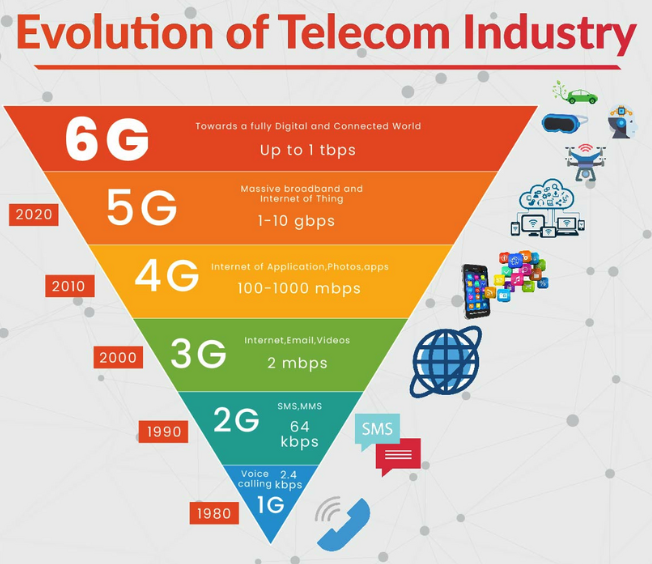
\includegraphics[width=\linewidth]{images/evolution.png}
    \caption{Evolution of Telecom Technologies}
    \label{fig:telecom-evolution}
\end{figure}

\section{Trending Technologies}
The seminar discussed several key technologies that are driving the digital transformation of industries and shaping the future of the digital economy. These technologies include:

\subsection{5G}
5G networks are the next generation of wireless technology that promises faster data speeds, lower latency, and greater capacity than previous generations. 5G networks are expected to enable a wide range of applications, including autonomous vehicles, smart cities, and the Internet of Things. The seminar highlighted the transformative potential of 5G technology and its implications for various industries.
\par Standalone 5G deployment consists of user equipment — the RAN and NR interface — and the 5G core network, which relies on a service-based architecture framework with virtualized network functions. Network functions that usually run on hardware become virtualized and run as software.
5G enables applications such as autonomous driving, remote surgery, and smart infrastructure. Figure \ref{fig:5g-applications} showcases some key use cases of 5G technology.

\begin{figure}[htbp]
    \centering
    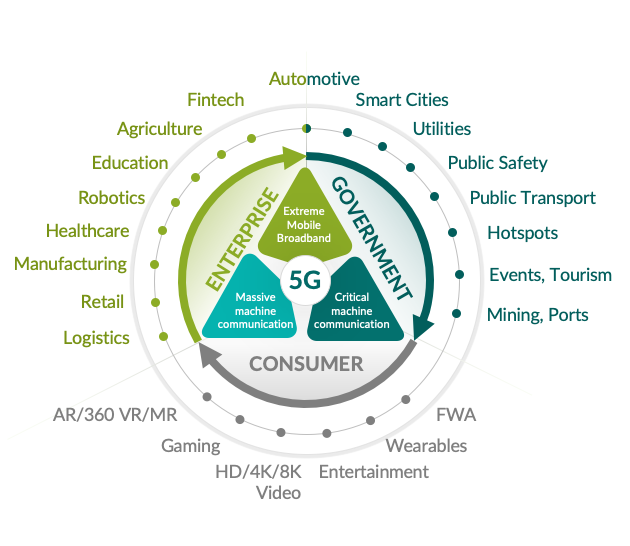
\includegraphics[width=\linewidth]{images/5g-applications.png}
    \caption{Some of the key applications of 5G technology}
    \label{fig:5g-applications}
\end{figure}

\subsection{Internet of Things (IoT)}
The Internet of Things (IoT) refers to the network of interconnected devices that can communicate and exchange data with each other. IoT devices can range from smart home appliances and wearables to industrial sensors and autonomous vehicles. \cite{DBLP:conf/iot/2023} The seminar discussed how IoT technology is transforming industries by enabling real-time monitoring, predictive maintenance, and data-driven decision-making. The seminar also addressed the challenges of IoT security and privacy and the need for robust cybersecurity measures to protect IoT devices and data. 
\begin{figure}[htbp]
    \centering
    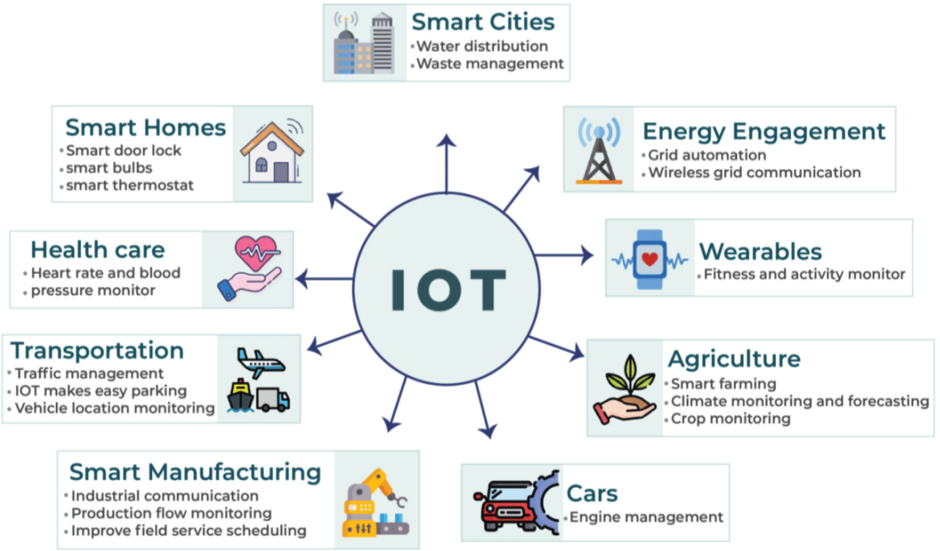
\includegraphics[width=\linewidth]{images/iot.png}
    \caption{Internet of Things (IoT)}
    \label{fig:iot}
\end{figure}

\subsection{Artificial Intelligence (AI)}
Artificial Intelligence (AI) refers to the simulation of human intelligence in machines that can perform tasks that typically require human intelligence, such as visual perception, speech recognition, and decision-making. The seminar discussed how AI technology is being used in various industries, including healthcare, finance, and manufacturing, to automate processes, analyze data, and improve efficiency. The seminar also addressed the ethical implications of AI and the need for responsible AI development and deployment. \cite{BALMER2020101977} AI-powered chatbots and virtual assistants are transforming customer service in the telecommunications sector. These tools provide instant responses to customer queries, handle routine tasks, and escalate complex issues to human agents, thereby improving customer satisfaction and reducing operational costs. 
\begin{figure}[htbp]
    \centering
    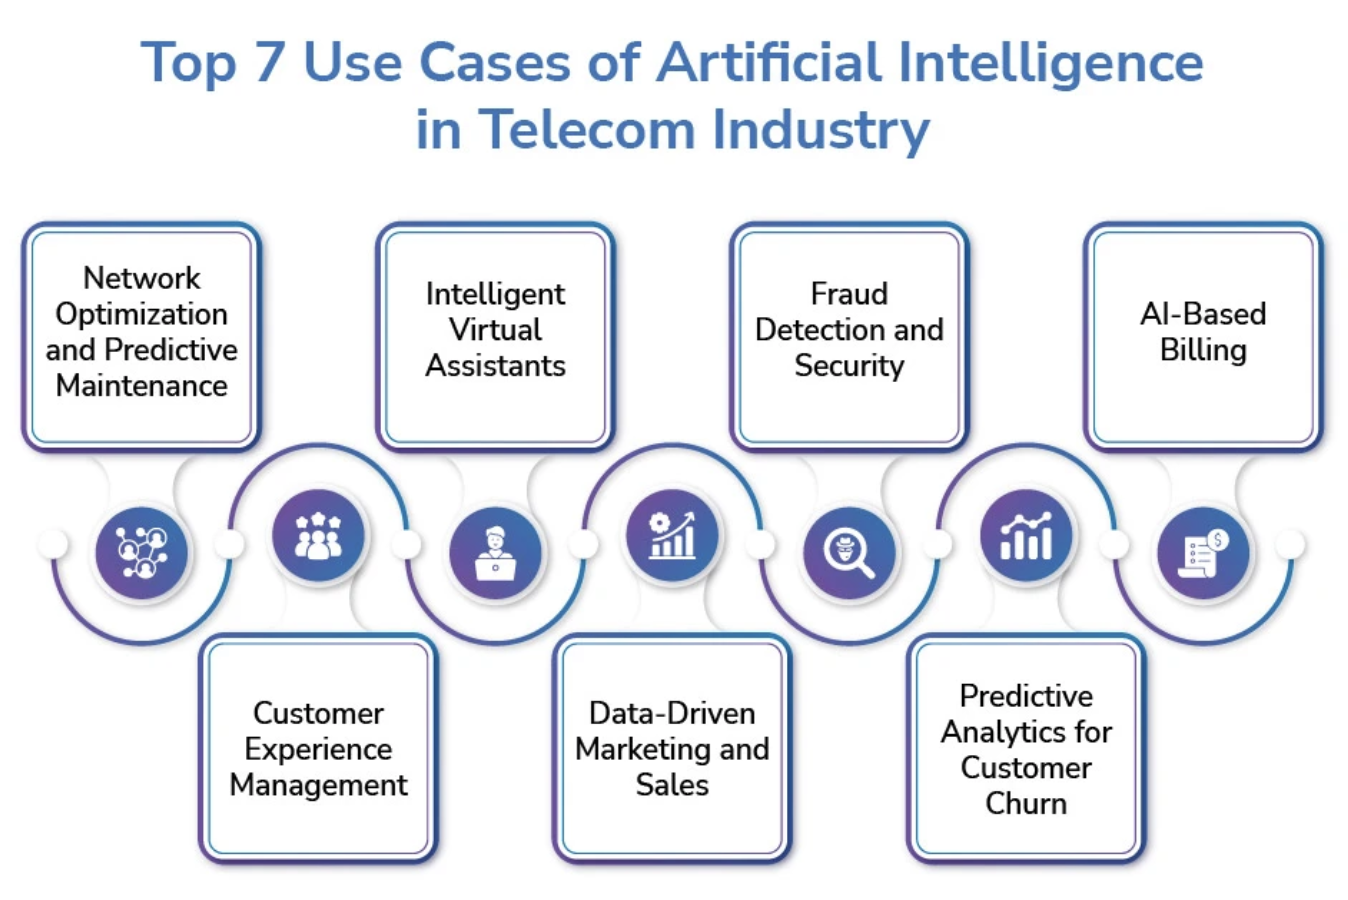
\includegraphics[width=\linewidth]{images/ai.png}
    \caption{AI on Telecom}
    \label{fig:ai-telecom}
\end{figure}

\subsection{Blockchain}
Blockchain is a decentralized, distributed ledger technology that enables secure and transparent transactions without the need for intermediaries. 
\begin{figure}[htbp]
    \centering
    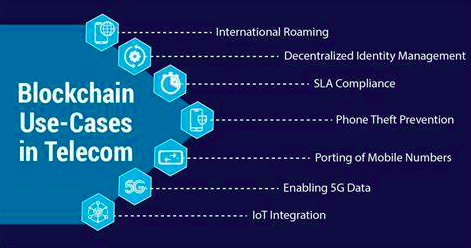
\includegraphics[width=\linewidth]{images/blockchain.png}
    \caption{Blockchain on Telecom}
    \label{fig:blockchain-telecom}
\end{figure}
The seminar discussed how blockchain technology is being used in various industries, including finance, supply chain, and healthcare, to streamline processes, reduce fraud, and increase trust. The seminar also addressed the challenges of blockchain scalability and interoperability and the need for standards and regulations to govern blockchain applications. \cite{magedanz1996intelligent} Blockchain technology is transforming the telecommunications industry by enabling secure and transparent transactions, reducing fraud, and improving trust between parties. Telecom companies are exploring blockchain applications in areas such as identity management, supply chain, and billing to enhance security, efficiency, and transparency. In telecommunications, blockchain can streamline processes such as identity management and fraud detection. It also enhances the security of data transactions.


\section{Impact on Digital Economy}
The digital economy encompasses all economic activities that rely on digital technologies. It is characterized by the widespread use of digital platforms and services.
Telecom technologies such as 5G, IoT, and blockchain are driving the growth of the digital economy by enabling new business models and enhancing productivity.
Digital technologies are transforming traditional business models, creating new opportunities for innovation and growth.
\begin{figure}[htbp]
    \centering
    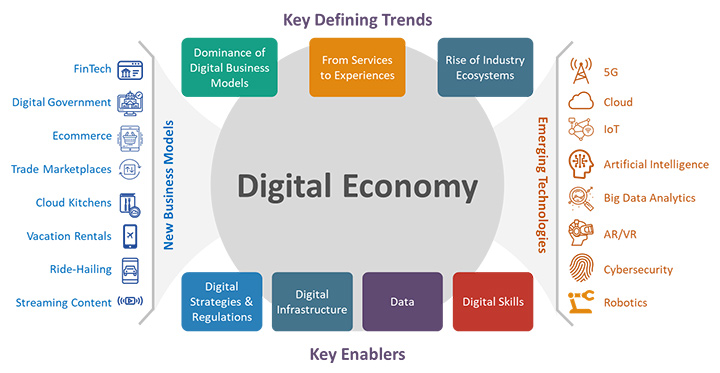
\includegraphics[width=\linewidth]{images/digital-economy.jpg}
    \caption{Technology and Digital Economy}
    \label{fig:digital-economy}
\end{figure}
\par The digital economy offers numerous opportunities for economic growth. However, it also presents challenges such as digital divide and cybersecurity threats. Addressing these challenges is crucial for sustainable development.

\section{Conclusion}
Telecom technologies are at the forefront of the digital transformation, driving significant changes in the economy. The seminar highlighted the importance of continuous innovation and collaboration among stakeholders to leverage these technologies for economic growth. Future advancements in telecom will further enhance connectivity, efficiency, and security, shaping the future of the digital economy. By embracing emerging technologies and fostering a culture of innovation, businesses and governments can unlock new opportunities and drive sustainable growth in the digital economy. The seminar provided valuable insights into the transformative potential of telecom technologies and their impact on the digital economy, underscoring the need for strategic investments and policies to harness these technologies for inclusive and sustainable development. 

\section*{Acknowledgment}
I would like to thank Prof. Dr. Pradip Paudyal for his invaluable insights and guidance during the seminar. Special thanks to the Department of Computer Science and Multimedia at Phoenix College of Management for organizing the seminar. Gratitude is also extended to Lincoln University for its support and to all participants who contributed to the fruitful discussions.
 
\bibliographystyle{IEEEtran}
\bibliography{references}

\end{document}